\documentclass{article}
\usepackage{asymptote}
\usepackage[utf8]{inputenc}
\usepackage{amsmath}
\usepackage{mathtools}
\usepackage{esint}
\usepackage{tikz}
\usepackage{float}
\usepackage{bm}
\usetikzlibrary{matrix,arrows,calc}
\usepackage{graphicx}
\usepackage{breqn}
\usepackage[margin=0.5in]{geometry}
\usepackage{array}
\usepackage{calc}
\usepackage{dsfont}

\usepackage{tikz}
\usepackage{tikz-3dplot}

\DeclareMathOperator*{\argmin}{arg\,min}
\DeclareMathOperator*{\argmax}{arg\,max}

\newlength\celldim \newlength\fontheight \newlength\extraheight
\newcounter{sqcolumns}
\newcolumntype{S}{ @{}
>{\centering \rule[-0.5\extraheight]{0pt}{\fontheight + \extraheight}}
p{\celldim} @{} }
\newcolumntype{Z}{ @{} >{\centering} p{\celldim} @{} }
\newenvironment{squarecells}[1]
{\setlength\celldim{2em}%
\settoheight\fontheight{A}%
\setlength\extraheight{\celldim - \fontheight}%
\setcounter{sqcolumns}{#1 - 1}%
\begin{tabular}{|S|*{\value{sqcolumns}}{Z|}}\hline}
% squarecells tabular goes here
{\end{tabular}}

\newcommand\nl{\tabularnewline\hline}


\newcounter{sarrow}
\newcommand\xrsquigarrow[1]{%
\stepcounter{sarrow}%
\begin{tikzpicture}[decoration=snake]
\node (\thesarrow) {\strut#1};
\draw[->,decorate] (\thesarrow.south west) -- (\thesarrow.south east);
\end{tikzpicture}%
}


\DeclareMathOperator{\sign}{sign}
\DeclareMathOperator\erf{erf}
\DeclareMathOperator\erfinv{erf^{-1}}

%\DeclareMathOperator*{\argmin}{arg\,min}

\title{Video Rectangle Tracking}
\author{charles dunn}
\date{\today}

\begin{document}

\maketitle

\section{Problem}

The goal of this project was to create an algorithm that tracks a rectangle in a video file. The inputs are a video with moderate shakiness and a rectangle specified by $(x,y)$ pixel coordinates from the top left corner, width $w$ and height $h$, all for the first frame.

In the sample videos provided, and perhaps unsurprisingly considering Uru's product, the rectangle is on a flat, blank wall. There are some discernible objects in view, like a TV and a door.

\section{Approach}

\subsection{Sparse Feature Correspondence}

Typical object tracking relies on obvious features of the object, such as text or sharp corners. FAST, MSER, BRISK, SURF, and SIFT feature detection algorithms all attempt to reduce the dimensionality of frame correspondence by identifying unique regions of an image. Ideally, a video input would have enough blobs, edges, or corners to enable tracking sparse features from one of the algorithms mentioned. One could then use a feature matching algorithm and RANSAC to derive a reasonable transformation from one frame's features to the next. 

In the case of the video inputs given, low resolution, blurriness, and insufficient detail in the scene prohibited reliably producing a reasonable homographic transformation. Even after lowering the feature detection thresholds, attempting homographic transform regularization, and smoothing final pixel shifts of the rectangle, sparse feature correspondence was unable to produce a stable solution. The solutions were still jittery at best, and often experienced instabilities.

\subsection{Dense Correspondence}

I then decided dense correspondence would be a better approach for the specific videos provided. This initially seemed to be much more computationally intensive that sparse features. The basic approach is to simply find the $x$ and $y$ offsets between each adjacent frame. There are a few different metrics commonly used, typically the sum of squared differences (SSD) or sum of absolute differences (SAD). I opted to use SSD on the gradient of the frames. 

I used the gradient, instead of the raw frame, because I was worried that the noise in large, flat areas of the video would dominate an offset search, and that shadows in the video would lead to large errors. The gradient, however, denotes edges and corners where tracking is less ambiguous. In a way, using dense correspondence on the gradient image is a middle ground between sparse and dense correspondence. Second, calculating the gradient helped with finding angle offsets later.

Let $R_n,G_n,B_n$ be the red, green, and blue color values for frame $n$ and let $(i,j)$ be pixel coordinates. Using the standard image gradient function, I can calculate $g_n$ for each pixel of each frame.

\begin{equation}
g_n(i,j) = \left |\left |\nabla \frac{R_n(i,j) + G_n(i,j) + B_n(i,j)}{3}\right|\right|
\end{equation}

We can now calculate the sum of squared differences for each frame $D_n$ for each horizontal and vertical pixel offsets $(x,y)$ within a certain range.

\begin{equation}
D_n(x,y) = \sum_{i=1}^w \sum_{j=1}^h (g_n(i+x,j+y)-g_{n-1}(i,j))^2
\end{equation}

Our desired final pixel offsets $(x^*_n,y^*_n)$ should minimize our SSD function.

\begin{equation}
(x^*_n,y^*_n) = \argmin_{x,y} D_n(x,y)
\end{equation}

In short, by using the gradient images, I hoped to find a minimum in the SSD between the previous frame and a shifted version of the current frame. Calculating the SSD for integer offsets within a pixel offset region was extremely slow, as one might expect, even for a reasonable search space of $32$ pixels in each direction. I therefore made the assumption of convexity within a small region. This is equivalent to assuming only small shifts between frames, or assuming input video without extreme shaking or motion. Figure 1 shows a plot of the SSD function between frames 1 and 2 of video1.mp4.

\begin{figure}
  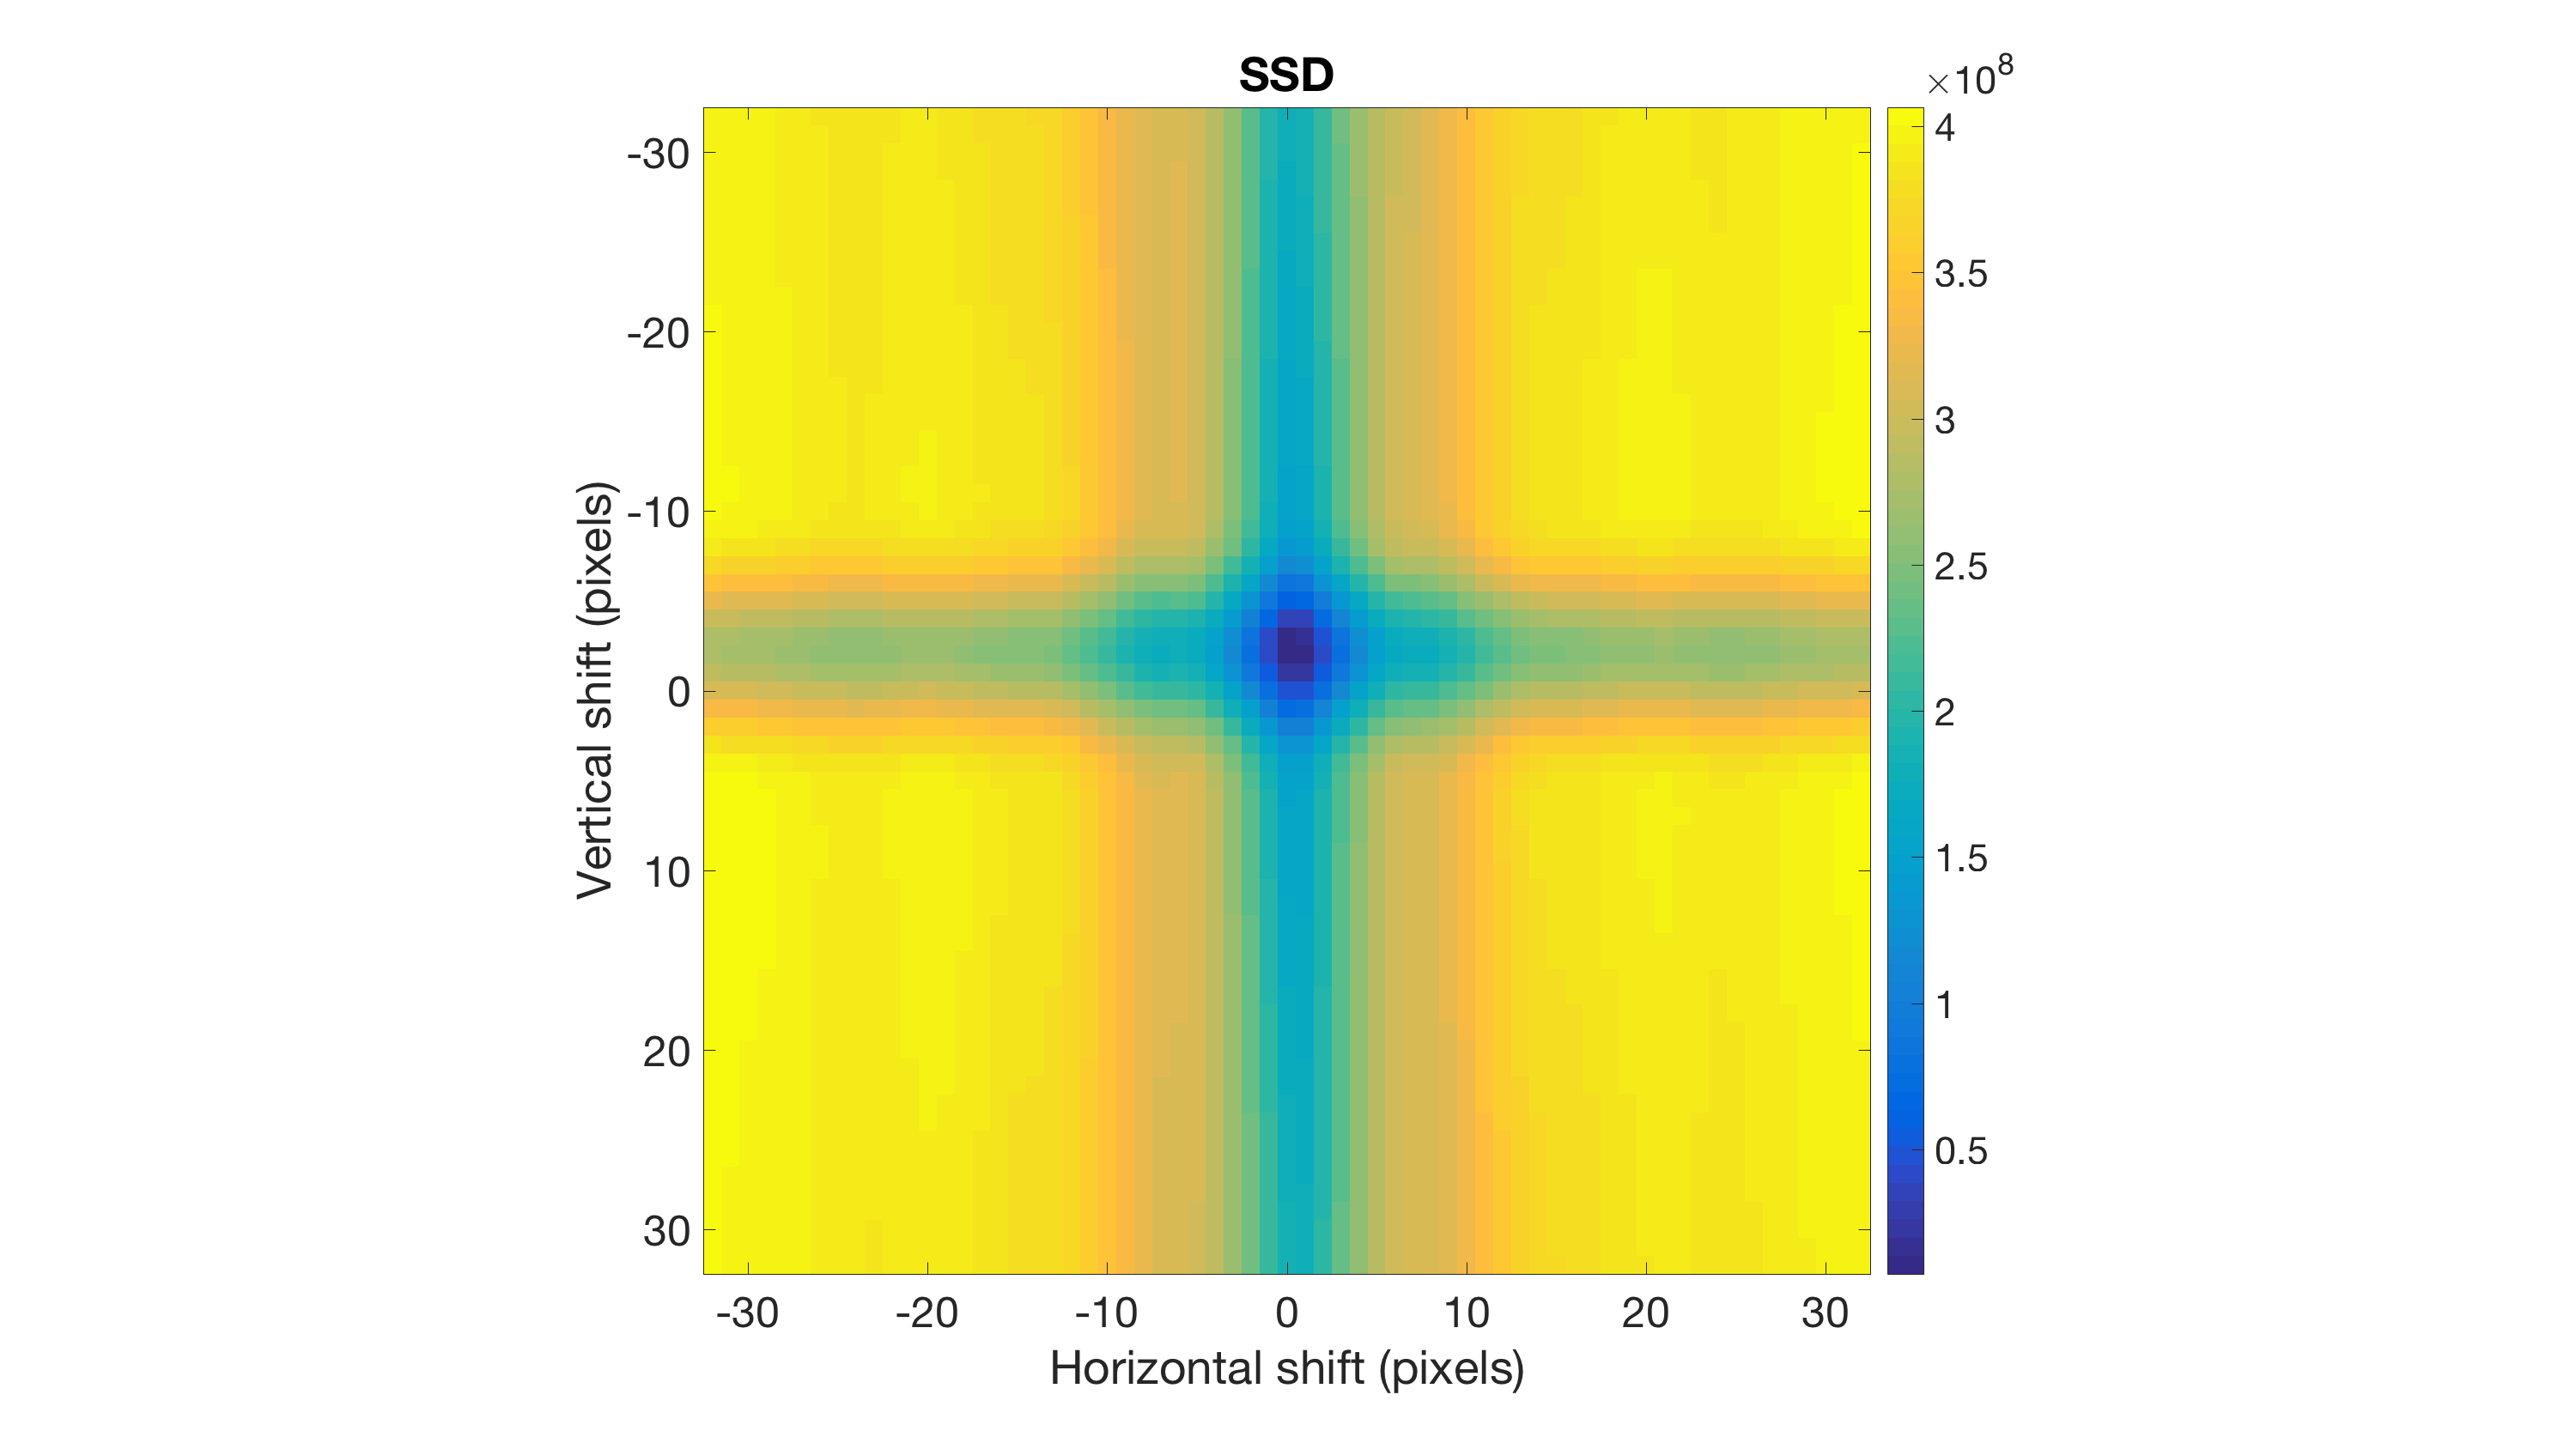
\includegraphics[width=\linewidth]{SSD_plot.png}
  \caption{The SSD function shows strong convexity near $(0,0)$.}
  \label{fig:boat1}
\end{figure}
\begin{figure}
  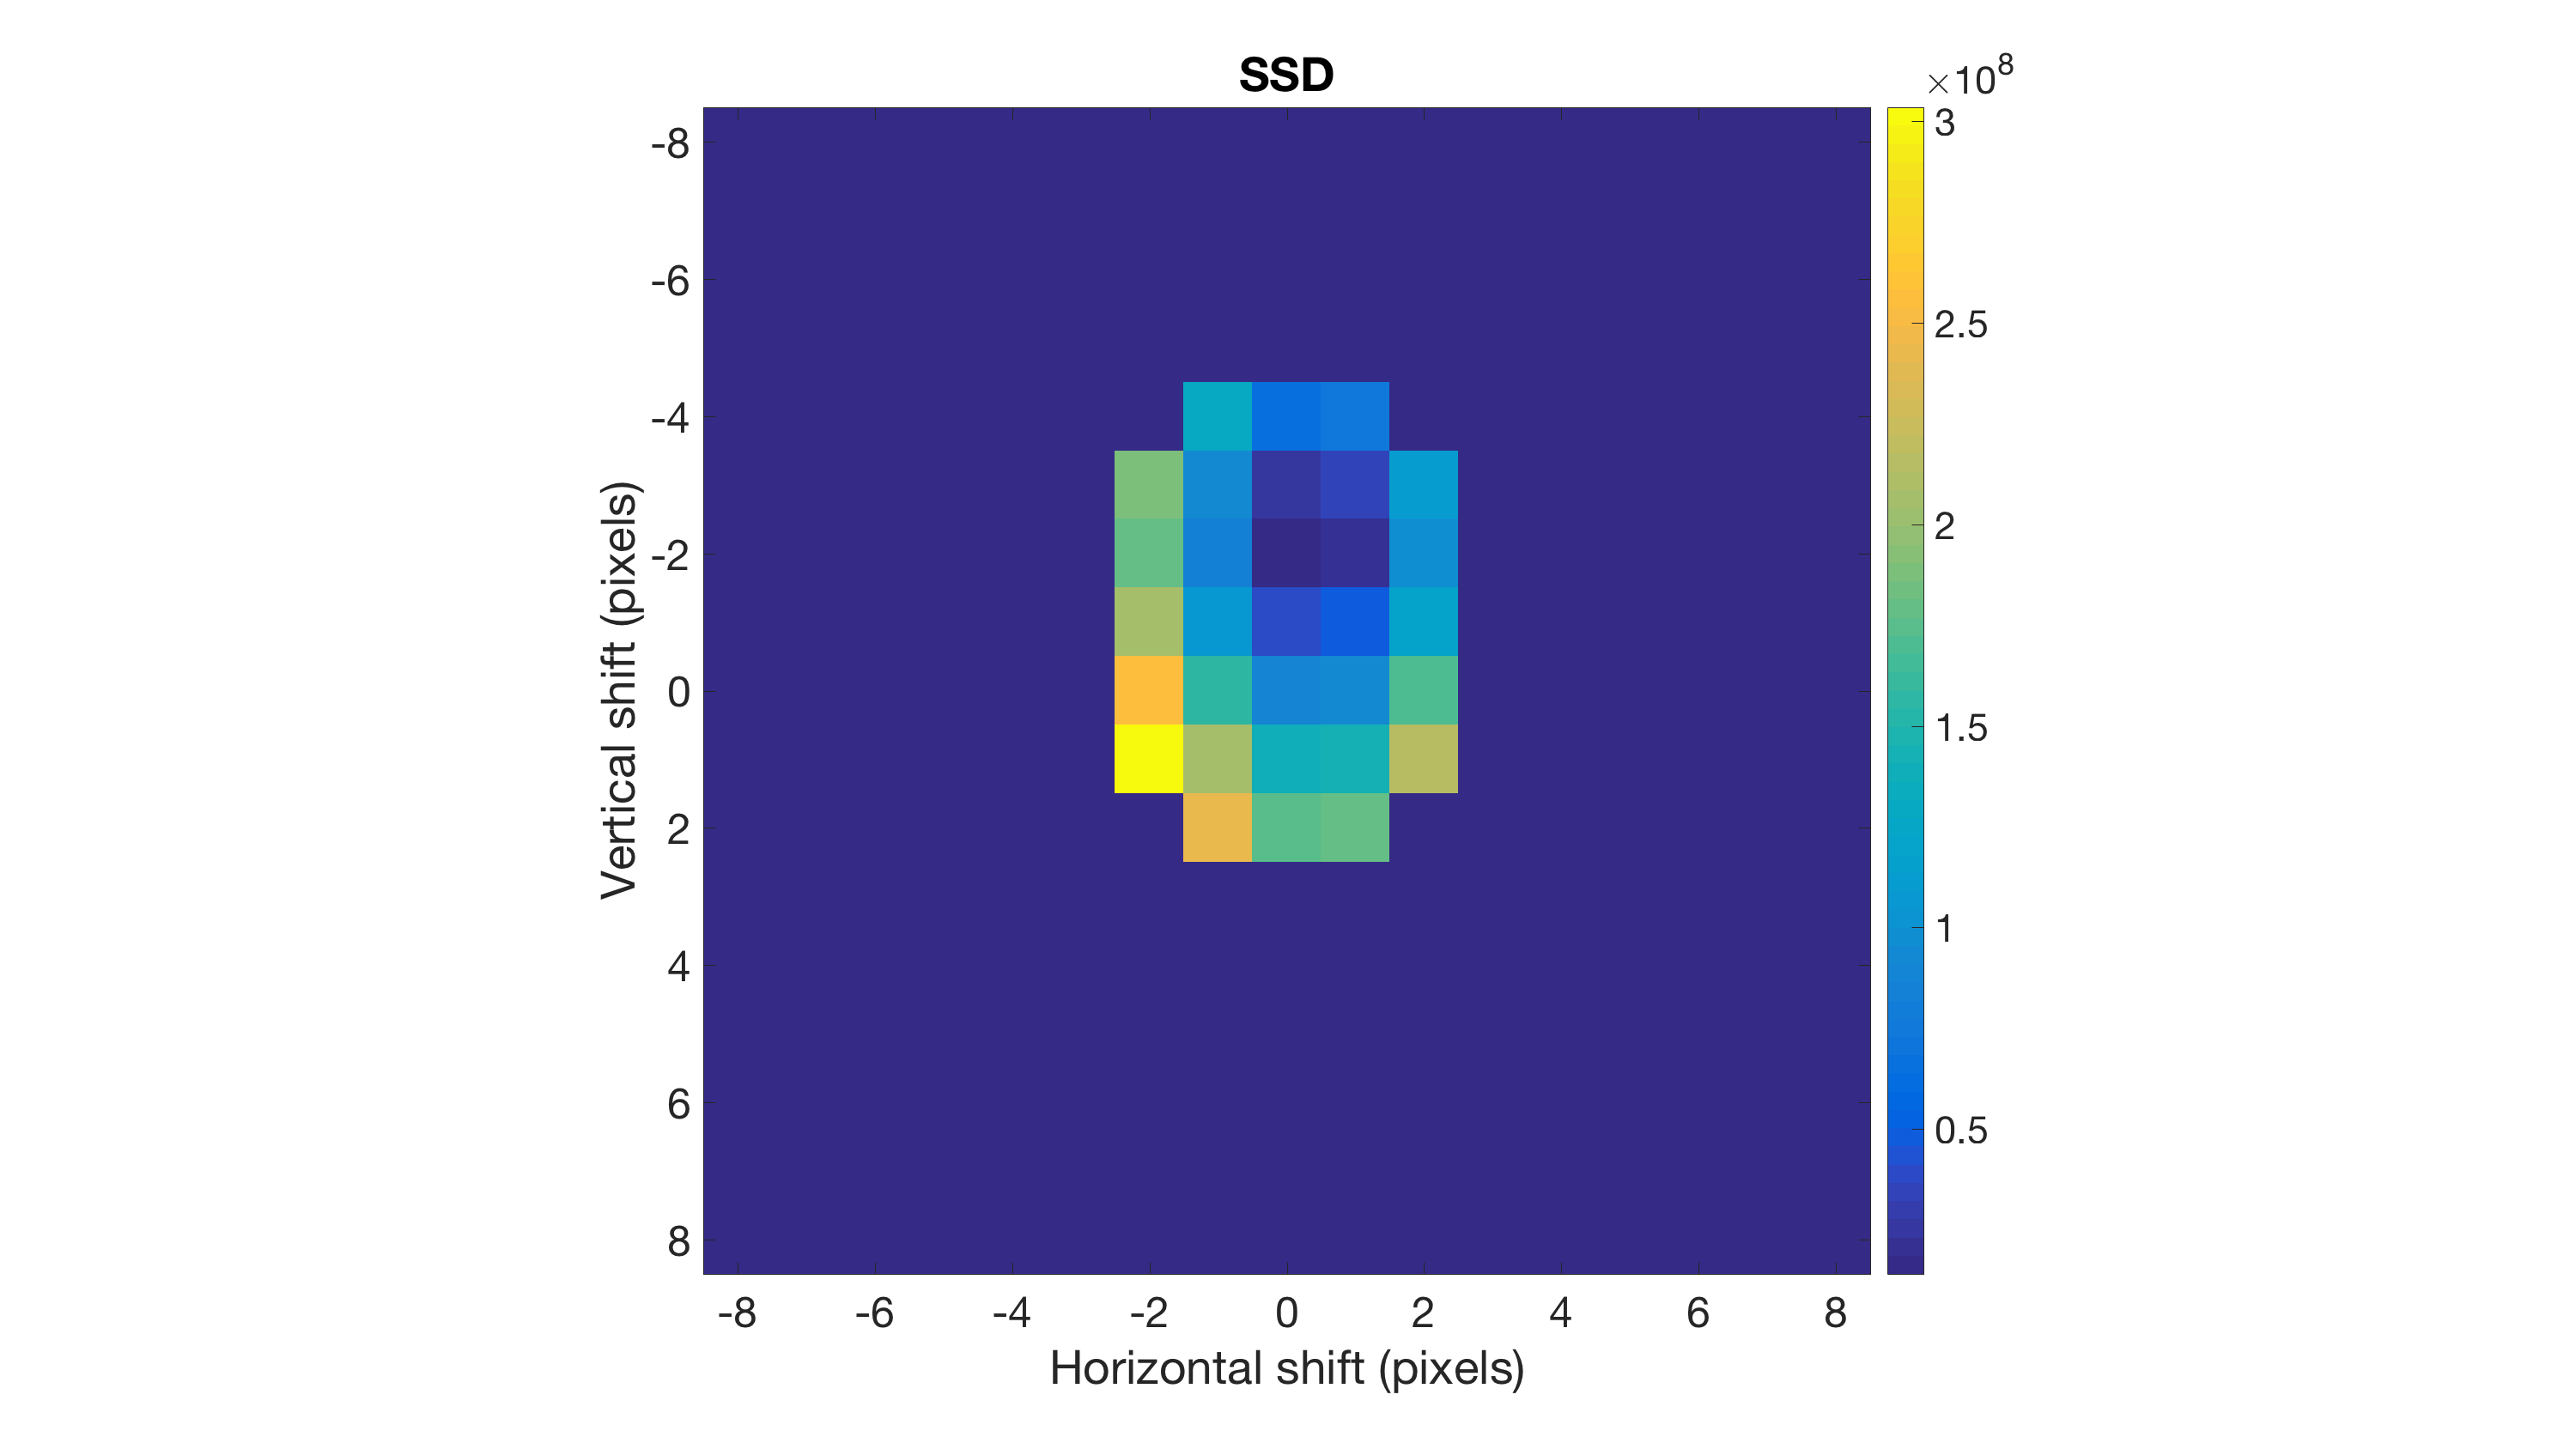
\includegraphics[width=\linewidth]{SSD_GD_plot2.png}
  \caption{The SSD function for frame 2 using "gradient descent".}
  \label{fig:boat1}
\end{figure}

With the assumption of convexity for the region of small offsets, I search the SSD space over each integer pixel offset by a numerical gradient descent of sorts. I initialize my search by the offset of the previous frame (employing the assumption that the camera frame rate is higher than the changes in direction of the camera), and search a small region around my initial point. I then find the minimum in my SSD function, and again search in a small region around this new point. I check if the SSD has already been calculated for any pixel offset to avoid repeated computation. I limit the offset to be $\pm32$ pixels in any one direction. Figure 2 shows center of the SSD for a few frames of video1.mp4 after using my gradient descent method. Note that most of the space is uncalculated since I had already found a local minimum.

After finding the local minimum in pixel shifts, I move the previous frame's rectangle corner coordinates by the same amount. Now that translation is mostly accounted for, I estimated any rotation of the video frame by looking at the distribution of angles of strong gradients. By matching histograms of the gradient angles for each frame, I got an approximate measure of rotation of the video, frame by frame. Most of the angle offsets detected were very small.

\section{Performance}

For video1.mp4 and video2.mp4 (30fps, 720p color), a my algorithm runs at about 5x realtime on a 2015 2.5 GHz Intel Core i7 MacBook Pro. The result for video1.mp4 is acceptable, with the rectangle tracking large and small jitters in the video. Rotation of the rectangle looks poor compared with the wall it is on in the video. Skew and scale are not accounted for at all. I didn't feel my algorithm was successful enough to tailor it to account for possible temporary occlusions as in video2.mp4, and the effect is large angle errors. Surprisingly, the pixel offset is already somewhat robust to the occlusions in this case.

\section{Improvements}

There is a lot of room for improvement. I still believe estimating a full homographic transformation matrix is required for a solution that accurately tracks a flat rectangle in a video. Some compromise between sparse and dense correspondences could still be used - perhaps by doing dense correspondence around strong detected feature points. I also believe that it is possible to leverage the lines in the videos more. Some feature sets are designed to find corners and others blobs, but for the particular videos provided, a feature set that includes lines would be very useful.

Another large shortcoming of the dense correspondence algorithm I propose is that it finds a global offset. In a video with surfaces that are at much different depths, feature points will not all move with the same transformation due to parallax and perspective. One way to avoid this would be to try to identify the surface behind the rectangular region first, or to simple take feature points or pixels that are relatively near the rectangular region, with the hope of only including points that are on the same plane as the rectangular region in 3D space.

The algorithm is quite slow, but potential speedups abound. A tiling approach would allow for homography estimation from dense correspondences while also preparing the algorithm for easy parallelization. Similarly, the algorithm could find the SSD minimum faster if a pyramidal approach was taken.

There could also be preprocessing steps to reduce the effects of noise and blurriness on the final result. During my attempt to use sparse features, I discovered that some frames with more camera movement had a significant decrease in sharpness (notably at the edge of the TV), which led to very few matches between frames.

In order to successfully track the rectangle in video2.mp4, with a few frames of occlusion, I believe foreground or movement identification would be required. Something simple like skipping frames that have large total differences would be a good first pass, but identifying motion of occluding objects by thresholding frame differences would be even better.

\section{Conclusion}

Please see the output videos (video1_out.avi and video2_out.avi) to see the performance of my final algorithm. I am excited to present my solution in person and discuss the project more. This was a fun project!


\end{document}
